% Win-informed column replication, toy example (9 columns, 3 workers, k=2).
\definecolor{twcTeal}{HTML}{1D9E75}%
\definecolor{twcCoral}{HTML}{D85A30}%
\definecolor{twcPurple}{HTML}{7F77DD}%
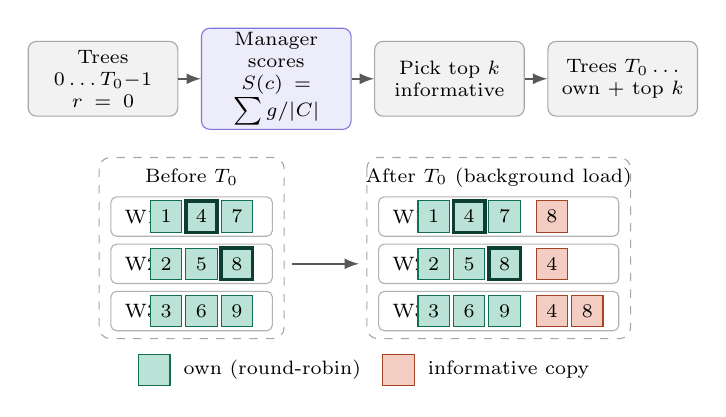
\begin{tikzpicture}[x=1cm,y=1cm,>=latex,
  twcstep/.style={draw, rounded corners=3pt, minimum width=1.9cm, minimum height=0.95cm,
    text width=1.75cm, align=center, font=\scriptsize, inner sep=1.5pt},
  gstep/.style={twcstep, draw=gray!70, fill=gray!10},
  pstep/.style={twcstep, draw=twcPurple, fill=twcPurple!14},
  panel/.style={draw=gray!70, dashed, rounded corners=4pt},
  worker/.style={draw=gray!60, fill=white, rounded corners=2pt},
  sq/.style={minimum size=0.4cm, inner sep=0pt, font=\scriptsize},
  own/.style={sq, draw=twcTeal!70!black, fill=twcTeal!30},
  cpy/.style={sq, draw=twcCoral!75!black, fill=twcCoral!30},
  plain/.style={},
  inf/.style={line width=1.3pt, draw=twcTeal!40!black}]
% top row: the four steps, only the manager step is purple
\node[gstep] (s1) at (0.95,0) {Trees $0\ldots T_0{-}1$\\$r=0$};
\node[pstep] (s2) at (3.15,0) {Manager scores\\$S(c)=\sum g/|C|$};
\node[gstep] (s3) at (5.35,0) {Pick top $k$\\informative};
\node[gstep] (s4) at (7.55,0) {Trees $T_0\ldots$\\own + top $k$};
\foreach \a/\b in {s1/s2, s2/s3, s3/s4} \draw[->, thick, gray!70!black] (\a.east) -- (\b.west);
% bottom row: dashed panels
\draw[panel] (0.9,-1.0) rectangle (3.25,-3.3);
\draw[panel] (4.3,-1.0) rectangle (7.65,-3.3);
\node[font=\scriptsize] at (2.075,-1.25) {Before $T_0$};
\node[font=\scriptsize] at (5.975,-1.25) {After $T_0$ (background load)};
\draw[->, thick, gray!70!black] (3.35,-2.35) -- (4.2,-2.35);
% worker boxes, stacked vertically
\foreach \y/\w in {-1.75/1, -2.35/2, -2.95/3} {
  \draw[worker] (1.05,\y-0.25) rectangle (3.1,\y+0.25);
  \node[anchor=west, font=\scriptsize] at (1.1,\y) {W\w};
  \draw[worker] (4.45,\y-0.25) rectangle (7.5,\y+0.25);
  \node[anchor=west, font=\scriptsize] at (4.5,\y) {W\w};
}
% own columns (round-robin), identical before and after
\foreach \y/\cols in {-1.75/{1/plain,4/inf,7/plain}, -2.35/{2/plain,5/plain,8/inf}, -2.95/{3/plain,6/plain,9/plain}} {
  \foreach \c/\s [count=\i from 0] in \cols {
    \node[own,\s] at (1.75+0.45*\i,\y) {\c};
    \node[own,\s] at (5.15+0.45*\i,\y) {\c};
  }
}
% informative copies, set apart from the own columns
\node[cpy] at (6.65,-1.75) {8};
\node[cpy] at (6.65,-2.35) {4};
\node[cpy] at (6.65,-2.95) {4};
\node[cpy] at (7.1,-2.95)  {8};
% legend
\node[own] at (1.6,-3.7) {};
\node[anchor=west, font=\scriptsize] at (1.85,-3.7) {own (round-robin)};
\node[cpy] at (4.7,-3.7) {};
\node[anchor=west, font=\scriptsize] at (4.95,-3.7) {informative copy};
\end{tikzpicture}
